\begin{center}
	\textbf{\LARGE{Metoda končnih elementov, ki minimizira kvadrat ostanka aproksimacije (\texttt{LSFEM})}}\\[0.25cm]
	\large{Seminarska naloga pri Naprednih numeričnih metodah}\\[0.7cm]
\end{center}

Numerično reševanje parcialnih diferencialnih enačb (\texttt{PDE}) je zaradi pomanjkanja vsestranskega algoritma še zmeraj bolj umetnost kot ustaljena znanost \cite{JiangB-LSFEM}. Pri zapletenih problemih hitro prispemo do vznožja gore matematične teorije, ki je ni moč zaobiti. Zaradi množice različnih pristopov reševanja ter raztresene in neprijazno napisane literature, lahko le ugibamo, kako visoko se bomo na poti do prelaza morali povzpeti. Zapletenim problemom prostorske dinamike v:
\begin{center}
	\begin{tabular}[h]{lll}
		\tabitem dinamiki tekočin,\hspace{1cm}	&	\tabitem termodinamiki,\hspace{2.5cm}	&	\tabitem elektrodinamiki,\\
		\tabitem kvantni teoriji,	&	\tabitem splošni teoriji relativnosti,&	\\
	\end{tabular}
\end{center}
kjer naletimo na \texttt{PDE}, se tako tudi v višjem izobraževanju najraje izognemo. Metoda končnih elementov (\texttt{FEM}), ki minimizira kvadrat ostanka aproksimacije (\texttt{LSFEM} = Least Squares \texttt{FEM}), obeta razvoj vsestranskega algoritma za reševanje \texttt{PDE} in s tem približanje omenjenih problemov širšemu krogu raziskovalcev.

\section{Temelji \texttt{LSFEM}}
Kadar obravnavamo prostorsko dinamiko (npr.\ tok tekočine), lahko fizični prostor modeliramo kot 1, 2 ali 3-mnogoterost. Temelje \texttt{LSFEM} bomo polagali na splošnem primeru $d$-mnogoterosti, za ponazoritev pa na njih sproti gradili konkretni 2D primer.

\begin{wrapfigure}{r}{5.5cm}
	\vspace{-0.3cm}
	\centering
	\captionsetup{type=figure}
	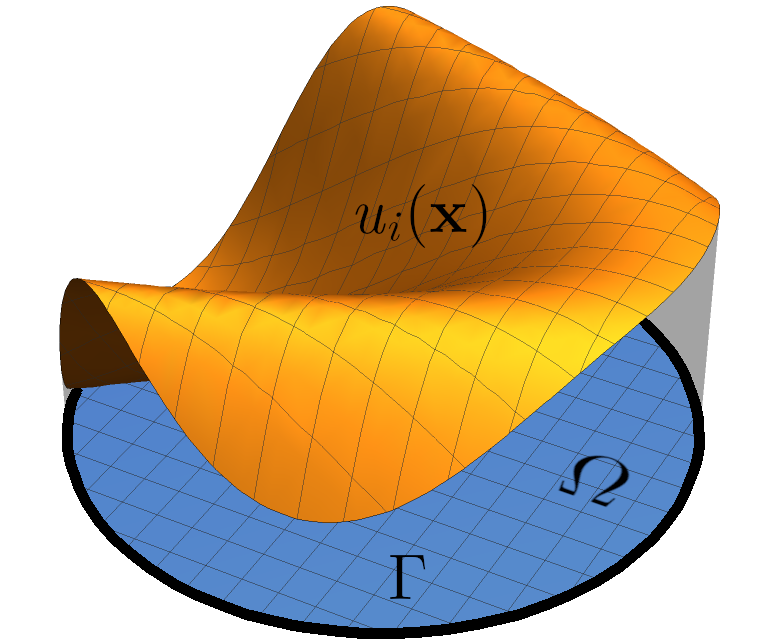
\includegraphics[width=5.5cm]{Slike/funkcijaInDomenaG}
	\caption{Domena $\Omega$, meja domene $\Gamma$ in komponenta rešitve $u_i(\mathbf{x})$.}
\label{fig:funkInDom}
\vspace{-2.6cm}
\end{wrapfigure}
Naj bo torej prizorišče dogajanja $d$-mnogoterost $\Omega$, opremljena s krajevnim vektorjem $\mathbf{x} = \{x_1, ..., x_d\}$. Pri reševanju sistema $m$ \texttt{PDE} iščemo nabor funkcij $\mathbf{u}(\mathbf{x}) =  \{u_1(\mathbf{x}), ..., u_m(\mathbf{x})\}$, ki v vsaki točki domene $\Omega$ zadosti sistemu \texttt{PDE}, na meji $\Gamma$ pa robnim pogojem (slika \ref{fig:funkInDom}). Konkretni primer bomo gradili na \textbf{sistemu Stokesovih enačb} za nestisljive tekočine v obliki \emph{u-p-$\omega$} (hitrost, tlak, vrtinčnost):\\[0.05cm]
\begin{minipage}{5.0cm}
\begin{IEEEeqnarray}{rl}
	\frac{\pd u}{\pd x} + \frac{\pd v}{\pd y} &= 0 \ , \\[0.3cm]
	\frac{\pd p}{\pd x} + \frac{\pd \omega}{\pd y} &= f_1 \ ,
\end{IEEEeqnarray}
\end{minipage}
\begin{minipage}{5.3cm}
\begin{IEEEeqnarray}{rl}
	\frac{\pd p}{\pd y} - \frac{\pd \omega}{\pd x} &= f_2 \ , \\[0.3cm]
	\omega - \frac{\pd u}{\pd y} - \frac{\pd v}{\pd x} &= 0 \ .
\end{IEEEeqnarray}
\end{minipage}\\[0.4cm]
To je le sistem stacionarnih Navier-Stokesovih enačb brez nelinearnih konvektivnih členov, ki jih moramo pri numeričnem reševanju linearizirati. Ker ta korak za ponazoritev \texttt{LSFEM} ni ključen, se mu na tak način izognemo. Kot zanimivost navržimo, da Stokesove enačbe opisujejo plazeče se tokove, pri katerih je konvekcija gibalne količine (zaradi gibanja) majhna v primerjavi z njeno difuzijo (zaradi viskoznosti). V enačbah ni časovnih odvisnosti (razen preko časovno odvisnih robnih pogojev), zato so takšni tokovi časovno obrnljivi: časovno obrnjena rešitev enačb je prav tako rešitev (slika \ref{fig:TaylorCouette}).

\begin{figure}[ht]
	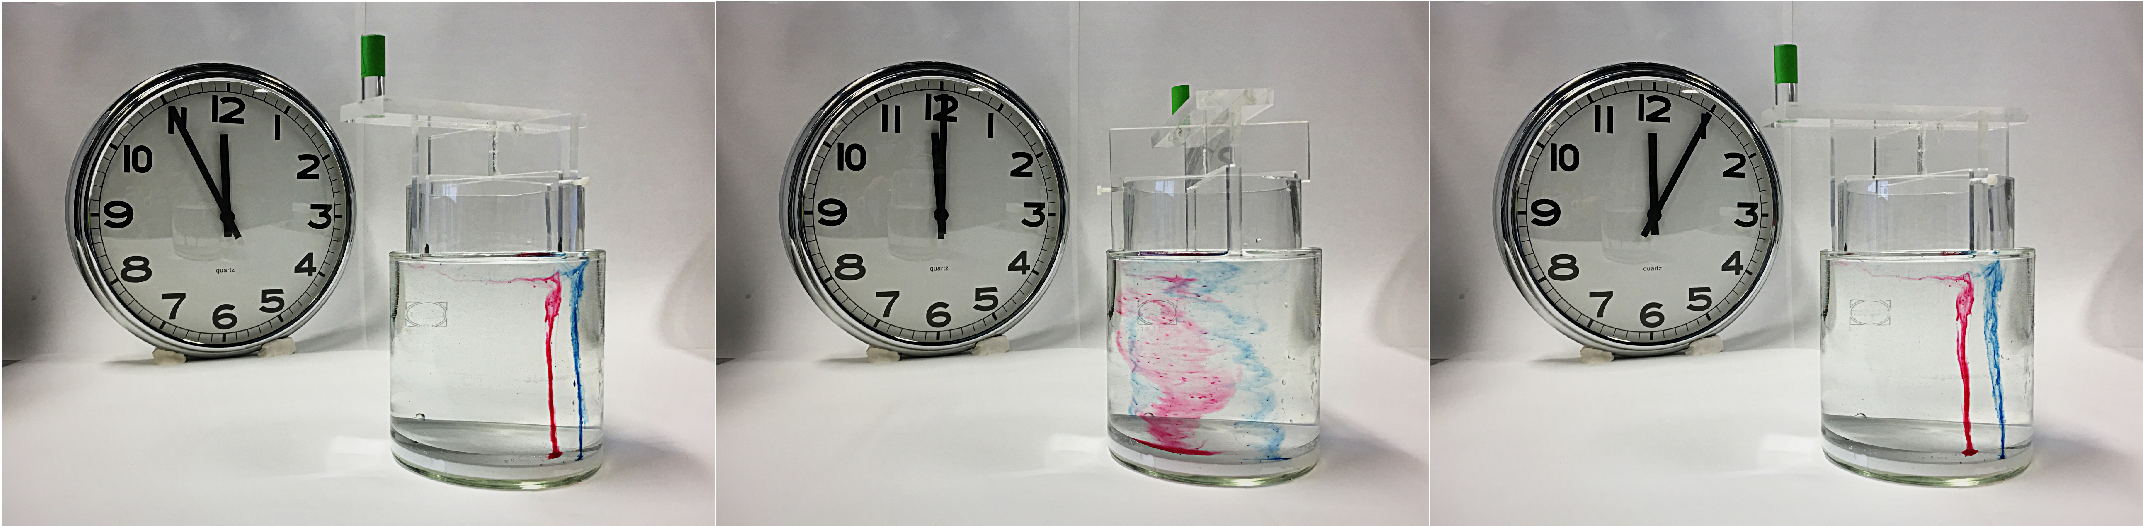
\includegraphics[width = 1\textwidth]{Slike/TaylorCouette}
	\caption{Zabaven eksperiment, pri katerem se v ozkem prostoru med dvema koncentričnima valjema nahaja viskozna tekočina, ki jo na dveh mestih označimo z liso barvila. Valja pet minut vrtimo v nasprotnih smereh (Stokesov tok, ki tako nastane, imenujemo Taylor-Couettov tok), da se lisi pomešata, nato smeri vrtenja obrnemo in po petih minutah se lisi ponovno sestavita \cite{Wiki-StokesFlow}.}
	\label{fig:TaylorCouette}
	\vspace{-0.2cm}
\end{figure}

Vse različice \texttt{FEM} vsaj okvirno temeljijo na variacijskem pristopu, kjer ne operiramo neposredno na \texttt{PDE}, ampak jih najprej pretvorimo v enakovreden variacijski problem: omislimo si \textbf{poskusno funkcijo} $\mathbf{w}(\mathbf{x})$, ki jo napnemo nad domeno $\Omega$, in izberemo funkcional $I[\mathbf{w}(\mathbf{x})]$, ki za vsako $\mathbf{w}(\mathbf{x})$ vrne neko realno število. Za uspešnost variacijskega pristopa Kakršenkoli funkcional za rešitev problema ni dober: ko je $\mathbf{w}(\mathbf{x})$ enaka rešitvi, mora funkcional vrniti najmanjšo vrednost. Fizikalno najintuitivnejša izbira je potencialna energija sistema, zaradi česar je bila različica FEM, ki jo na tak način dobimo, razvita prva. Vzamemo energijski potencial $F\left(\mathbf{w}\right)$, ki ga integriramo po domeni $\Omega$:

\setlength{\textheight}{26.5cm}
\pagebreak
\setlength{\topmargin}{1.6cm}			% Header Top Margin Height
\setlength{\headheight}{0.0cm}
\setlength{\headsep}{0.0cm}			% Header Lower Margin Height	 Footer height
\fancyhf{}
\fancyfoot[C]{\thepage}
% Negative vspace set in figure above.
\begin{equation}
	I[\mathbf{w}(\mathbf{x})] = \int_{\Omega} F\left(\mathbf{w}(\mathbf{x})\right) \, \ud \Omega \hspace{1.4cm} \texttt{funkcional poskusne funkcije} \quad ,
	\label{eq:GeneralFunctional}
\end{equation}

kar je po definiciji potencialna energija sistema. Iščemo minimum funkcionala, zato poskusno funkcijo $\mathbf{w}$ razvijemo okoli rešitve $\mathbf{u}(\mathbf{x})$:
\begin{equation}
	\widetilde{\mathbf{w}}(\mathbf{x}, \varepsilon) = \mathbf{u}(\mathbf{x}) + \varepsilon \mathbf{v}(\mathbf{x}) \quad ,
\end{equation}
kjer je $\mathbf{v}(\mathbf{x})$ poljubna odmična funkcija, $\varepsilon$ pa realno število. Razvito funkcijo vstavimo v funkcional \eqref{eq:GeneralFunctional} in ga nato odvajamo po $\varepsilon$:
\begin{equation}
\frac{\ud I}{\ud \varepsilon} = \int_{\Omega} \frac{\ud}{\ud \varepsilon} F(\widetilde{\mathbf{w}}) \, \ud \Omega = \int_{\Omega} \frac{\ud F}{\ud \widetilde{\mathbf{w}}} \cdot \frac{\ud \widetilde{\mathbf{w}}}{\ud \varepsilon} \ \ud \Omega = \int_{\Omega} \frac{\ud F}{\ud \widetilde{\mathbf{w}}} \cdot \mathbf{v} \ \ud \Omega \quad .
\end{equation}

Fizikalno najintuitivnejša je \textbf{Rayleigh-Ritzeva različica}, kjer za $F$ uporabimo energijski potencial sistema \texttt{PDE}. Rešitev $\mathbf{u}(\mathbf{x})$ je potemtakem funkcija, ki minimizira totalno potencialno energijo sistema. Rayleigh-Ritzeva različica poseduje lastnost najboljšega približka (minimizira razliko energijskih norm numerične in eksaktne rešitve), hkrati pa vodi do sistema linearnih algebrajskih enačb, ki je zelo prikladen za reševanje s hitrimi iteracijskimi metodami.

Z Rayleigh-Ritzevo metodo dobimo sistem linearnih algebrajskih enačb za 

Galerkin, Najmanših kvadratov \cite{JiangB-LSFEM}
Basic lemma of variational principles: Temeljni lema variacijskih načel.

\textbf{Rayleigh-Ritzeva različica} \texttt{FEM}, ki je bila razvita prva in ima korenine v začetku dvajsetega stoletja (cite), je prav tako variacijska metoda.